\documentclass[10pt, a4paper]{article}
\usepackage{lrec2006}
\usepackage{graphicx}
\usepackage{todonotes}
\usepackage[hidelinks]{hyperref}

\newcommand{\lemon}[0]{\emph{lemon}}

\title{Publishing and Linking WordNet using Lemon and RDF}

\name{John P. M\textsuperscript{c}Crae\textsuperscript{$\diamondsuit$}, Christiane Fellbaum\textsuperscript{$\clubsuit$} and Philipp Cimiano\textsuperscript{$\diamondsuit$}}

\address{ \textsuperscript{$\diamondsuit$}University Bielefeld, \textsuperscript{$\clubsuit$}Princeton University \\
               CITEC Building, Inspiration 1, 33615 Bielefeld, Germany; 35 Olden Street, Princeton, USA \\
               \{jmccrae, cimiano\}@cit-ec.uni-bielefeld.de, fellbaum@princeton.edu \\}


\abstract{In this paper we provide a description of a dataset consisting of data
    from the Princeton WordNet. This version is intended to provide canonical
    URIs that can be used by a wide variety of lexical resources to express
    their linking as part of the Linguistic Linked Open Data Cloud.
    Furthermore, this is the first version to use
    the \lemon{} model and we describe how we represent WordNet with this model.
\\ \newline \Keywords{dataset description, language resources, lexicon, ontology, WordNet, linked data}}


\begin{document}

\maketitleabstract

\section{Introduction}

WordNet is still one of the most widely used lexical resources within natural 
language processing. From the time since the first version of WordNet was released, many
resources have been produced that represent complementary information to WordNet~\cite{schuler2005verbnet,baker1998berkeley}
or extend it to other languages~\cite{vossen1998eurowordnet,bond2013linking}. 
Meanwhile, new Web technologies, in particular Linked Data, have fostered the publication of data on the Web.
This has lead to the emergence of a so called \emph{Linguistic Linked Open Data (LLOD)} cloud in which resources and datasets are represented in RDF format and linked to each other.
Linked data, as proposed by \cite{berners2011linked}, has four
main principles for publishing data: firstly, that it relies on URIs to identify
objects; secondly, that these URIs should be resolvable; thirdly, that semantic
information is returned, using standards such as RDF and finally, that links are
provided to other resources. 
Recent activity in the context of the ontology-lexicon interface has
led to the creation of a number of models, most notably
\lemon{}~\cite{mccrae2012interchanging}, providing a principled method for publishing lexical data in combination with ontologies that define the semantics of the lexical entries.
Given the popularity and availability of WordNets in
many languages, it is important to clarify how WordNets can be integrated into the Linked Data cloud.

In this paper we describe our experience
in publishing WordNet following the linked data principles and using the \lemon{} model. While this is not
the first version of WordNet to be published as linked data~\cite{van2006conversion,mccrae2012integrating,graves2006data}, our 
version has several advantages: firstly that it is linked to many
resources, secondly that it uses an open model, \emph{lemon}, and, most importantly, that 
it is directly hosted by Princeton and will thus directly be automatically in sync with further releases of WordNet. 
As such we intend that this data will provide a central hub for the linkage of
not only many WordNets in many languages, thus enabling the visions of a Global
WordNet Grid~\cite{pease2008building}, but also for many other kinds of lexical resources. 

\section{Background}

\subsection{WordNet}

WordNet~\cite{miller1995wordnet,fellbaum1998wordnet,fellbaum2010wordnet} is a large lexical database of English nouns,
verbs, adjectives and adverbs. Word forms are grouped into more than 117,000 sets of
(roughly) synonymous word forms, so called \emph{synsets}. These are interconnected by bidirectional
arcs that stand for lexical (word-word) and semantic (synset-synset) relations, including
hyper/hyponymy (\emph{tree-oak}), meronymy (\emph{tree-branch}), antonymy
(\emph{long-short}) and various entailment relations (\emph{buy-pay, show-see, untie-
tie}).

WordNet's synsets and its network structure yield a rough measure of semantic similarity
among words and concepts in terms of synset membership as well as the number of arcs
separating synsets. Consequently, WordNet has become a popular tool for Word Sense
Disambiguation (WSD) and Natural Language Processing in general. WordNets have
been built for around 100 different languages. Most are mapped onto the Princeton
WordNet, enabling translation on the lexical level as well as cross-lingual WSD and
applications. WordNet continues to evolve both in terms of coverage and representation
of meaning. Recent enhancements include the addition of internet language and partially
compositional multi word units. Finally, WordNet has been mapped to formal ontologies, 
including SUMO~\cite{niles2003mapping} and KYOTO~\cite{vossen2014kyoto}.

\subsection{lemon}

\lemon{} is a model that has been proposed~\cite{mccrae2012interchanging} for the representation of
lexicons relative to ontologies. As such, this model is well suited to the
representation of semantic networks such as WordNet and defines many useful
features for linking a WordNet to wider objects in the Semantic Web. \lemon{}
models lexicons by means of a core consisting of the following elements:

\begin{itemize}
  \item A \emph{lexical entry} which represents a single word or multi-word
    unit.
  \item A \emph{lexical sense}, representing a meaning of that word, which
    contains a \emph{reference} to a concept in the ontology.
  \item \emph{Forms}, which are inflected version of the entry, and associated
    with a string \emph{representation}.
\end{itemize}

In fact, in previous work~\cite{eckle2014lemonuby} \lemon{} has been used not only to
represent WordNet but to integrate it with more syntactically sophisticated
resources such as VerbNet. As such \lemon{} shows potential to help in the
integration of lexical data across many levels and languages.

\subsection{Linguistic Linked Data}

The application of linked data technology to the representation of linguistics
resources has been spearheaded by the OKFN Working Group on Linguistics~\cite{chiarcos2011towards},
who has been documenting the progress of this project by means of a cloud
diagram showing all the linguistic resources available on Linguistic Linked Open Data Cloud as well as the links between these.

There are many key advantages to the use
of this technology for language resources; however the cloud has until now
lacked a central node. As WordNet is the most widely referenced language
resource, we believe that WordNet can act as a nucleus for linguistic linked data
in the way that DBpedia~\cite{auer2007dbpedia} has for the wider cloud.

Chiarcos et al. \cite{chiarcos2013towards} have discussed the
application to linguistic data and argue that this model has notable
advantages over standard approaches to data modelling, in particular the following:

\begin{enumerate}
    \item Representation: Graph-based models are a method that can represent any
        form of language resource.
    \item Structural interoperability: By using RDF graphs and URIs, datasets can
        be merged from a syntactic point of view straightforwardly.
    \item Federation: Multiple datasets can easily be drawn from different
        sources in the web and used together seamlessly.
    \item Conceptual interoperability: Linking to common data category
        repositories supports interoperability.
        \item Ecosystem: Building on standards such as RDF supports the use of common
        tools, including databases.
    \item Dynamic import: Data on the web is not static and as such errors can
        be corrected after publication.
    \item Expressivity: The use of other Semantic Web models allows the easy
        expression of metadata, provenance and ontological constraints on the
        data.
\end{enumerate}

\section{Representing WordNets with lemon}

\begin{figure}
    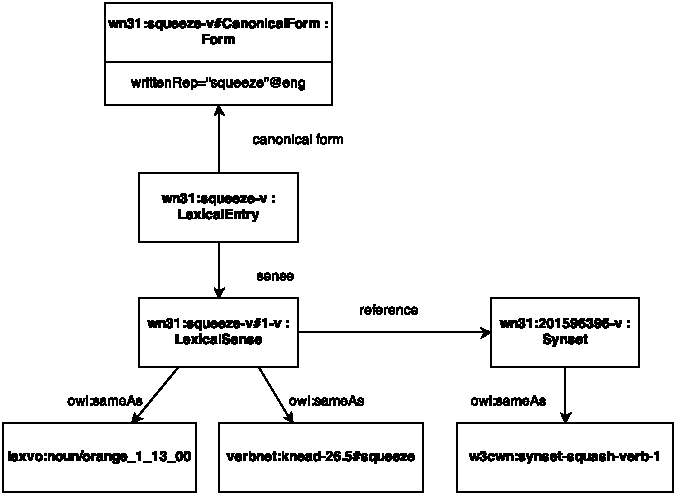
\includegraphics[width=0.5\textwidth]{wn-rdf-example}
    \caption{An example of the modelling a single word and synset and links to
        other resources\label{modelling_example}}
\end{figure}


%\begin{figure*}
%\caption{URI scheme of RDF WordNet\label{uri-examples}}
%\end{figure*}

\begin{table}
  \begin{tabular}{p{50mm}|c}
     & Number of triples \\
    \hline
    Links to VerbNet & 26,353 \\
    Links to LexVo & 458,907 \\
    Links to lemonUBY & 475,502 \\
    Links to W3C WordNet & 99,926 \\
    \hline
    Total & 8,903,345 \\
  \end{tabular}
  \caption{The number of links and total number of triples in
      WordNet-RDF\label{triple_counts}}
\end{table}

It is not trivial to apply \lemon{} to the case of a WordNet as there is no
clear ontology in WordNet.
Clearly, WordNet's 
words can be regarded as \lemon{} lexical entries and the word senses correspond
well to \lemon{}'s lexical senses. WordNet has lemmas and a separate list of
variants of these, and as such we create a canonical form for each lemma and another 
form for each of these variants. Since there is currently no indication in
WordNet of what grammatical properties these variants have, we do not attach additional properties to these variants/forms. As \lemon{} is a model for
ontology-lexica, the main question is what the reference of the lexical senses should be.
We choose to regard WordNet's synsets as ontological references, but instead of assigning them a formal ontological type (e.g.,
class, property or individual), we introduce a new type {\tt Synset} as a subclass of \emph{Concept} in SKOS~\cite{miles2007skos}.

This allows us to capture the nature of synsets without
ontologizing the semantic network as in~\cite{gangemi2003ontowordnet}.
Similarly, we introduce relations such as hypernymy, meronymy etc. as new
properties rather than attempt to relate them to existing ontological
properties such as OWL's subClassOf. In order to capture the new properties, we
introduce an ontology\footnote{\url{http://wordnet-rdf.princeton.edu/ontology}}
describing the new properties and classes and provide
axioms for the use in the context of both \lemon{} and SKOS. Furthermore, we
link the elements in the ontology to data categories from
ISOcat~\cite{kemps2008isocat} following the guidelines
of~\cite{windhouwer2012linking}.

Another key question concerns the identifiers we use for each element in the data.
We do not follow previous exports such as~\cite{van2006conversion} in assigning new identifiers
but instead attempt to use the existing identifiers in WordNet. Furthermore, as
WordNet has released several versions and is still under development, we consider it 
important to include the version number in the URI. As such, we use the
following scheme for URIs:, as exemplified below:

\begin{itemize}
  \item Each lexical entry is represented by means of the URL-encoded lemma and
    then a dash followed by the part of speech as a single letter (i.e., `n(oun)',
    `v(erb)', `a(djective)', `r (adverb)', `adjective s(atellite)' or `p(article)').    
    
  \item Senses and forms in the model use the entry URI and add a fragment identifier. For forms for which there is no previous identifier in WordNet, we
    use {\tt CanonicalForm} and {\tt Form-n} where {\tt n} is a number.
    For senses, the fragment is the index of the senses and the part of
    speech.
  \item Synsets are similarly are identified by a number consisting of 8 or 9 digits corresponding to offset codes in the WordNet database\footnote{The 9 figure codes
      include an extra initial digit for part-of-speech}, followed by a dash and the part of speech as a single letter.
\end{itemize}

Examples of this scheme include:

{\scriptsize
\begin{verbatim}
http://wordnet-rdf.princeton.edu/wn31/cat-n
http://wordnet-rdf.princeton.edu/wn31/cat-n#CanonicalForm
http://wordnet-rdf.princeton.edu/wn31/cat-n#2-n
http://wordnet-rdf.princeton.edu/wn31/300001740-a
\end{verbatim}}


A Python framework based on RDFlib\footnote{\url{https://github.com/RDFLib/rdflib}} is used to serve the website and
provide SPARQL access to the data.

\section{Linking WordNet}

In addition to providing a RDF/Linked Data version of WordNet, we have incorporated a number of links to other resources in the data. In particular
we include the following elements:

\begin{itemize}
  \item For verbs, we include mappings to VerbNet~\cite{schuler2005verbnet} if they exist. As
    VerbNet does not currently have a linked data version, we link to the
    PHP page of the web site.
  \item We include translations from the Open Multilingual WordNet~\cite{bond2013linking}
    collection as simple labels on the synsets, identified by the use of
    language codes.
  \item We have included previous mappings to LexVo~\cite{de2008language} 
    using the current identifiers in WordNet.
  \item We include links to the W3C WordNet 2.0 export~\cite{van2006conversion}.
  \item We have created new links to lemonUby~\cite{eckle2014lemonuby}.
\end{itemize}

In addition to these links, we provide support for legacy resources by
adding URL mappings from previous versions of WordNet identifiers to the most
recent version, with mappings based on \cite{daude2000mapping}. The number of
triples in the resource can be seen in table~\ref{triple_counts} and an example
of the data is illustrated in figure~\ref{modelling_example}.

\section{Related Work}

This work does not represent the first version of WordNet published in RDF. Previous versions
include the one by van Assem et al. \cite{van2006conversion} as well as McCrae et al. \cite{mccrae2012integrating}. Furthermore, WordNet has been
incorporated into various larger resources including
BabelNet~\cite{navigli2010babelnet,ehrmann2014} and 
UBY~\cite{gurevych2012uby,eckle2014lemonuby}. These projects however have mostly
been fixed to using a single version of WordNet. In contrast, we view our work
as more related to the task of providing universal identifiers for words as in the
ongoing work of the Global WordNet Grid~\cite{pease2008building}.  

There have been a number of attempts to interlink WordNets. 
\cite{pease2009formal} used an upper-level ontology called SUMO to group WordNet
concepts and these mappings are adopted by several language versions of WordNet.
Similarly, attempts were made to integrate WordNets based around the Kyoto
Ontology and LMF~\cite{soria2009wordnet}. Finally, the SemLink
project~\cite{palmer2009semlink} has
developed links among several resources, though it is not yet integrated into
the linked data cloud.

\section{Conclusion}

We have described a Linked Data version of Princeton WordNet that is expressed in RDF and linked to other relevant resources and furthermore is directly sychronized with the WordNet project.
Furthermore, we have discussed
the use of the \lemon{} model to describe a WordNet and ameliorate the
integration of not just other WordNets but also a wide variety of lexical
resources that are integrated with WordNet. We believe that our WordNet RDF model 
will constitute a key central node for the expansion of the Linguistic
Linked Open Data Cloud.

\bibliographystyle{lrec2006}
\bibliography{rdf-wordnet}

\end{document}
